%We begin by considering the following simple question: how close is the behavior of two given Markov chains $P$ and $Q$?
%A natural notion of distance would tell us how easy it is to distinguish which Markov chain $P$ or $Q$ a word $w=s_0\to s_1\cdots\to s_\ell$ of certain length $\ell$ was generated from. 
Given two Markov chains $P$ and $Q$, we want to come up with a distance notion which captures how easy it is to distinguish which Markov chain $P$ or $Q$ a word $w=s_0\to s_1\cdots\to s_\ell$ of certain length $\ell$ was generated from (while being agnostic to the distribution of $s_0$). 
This distinguishability is precisely captured by the TV distance $\dtv{\word{P}{\ell}}{\word{Q}{\ell}}$ between {\em word distributions} 
$\word{P}{\ell}$, $\word{Q}{\ell}$ for words of length $\ell$ generated by Markov chains $P$ and $Q$ respectively. It is more convenient in our setting to use, instead of total variation distance, the square of the Hellinger distance $\hellingersq{\word{P}{\ell}}{\word{Q}{\ell}}$
or the closely related Bhattacharya coefficient\footnote{Hellinger distance is tightly related to the Bhattacharya coefficient between two distributions which is defined as
$BC(p,q) = \sum_{i \in [k]} \sqrt{p_i\cdot q_i}$. It captures similarity of two distributions and lies in $[0,1]$.}, which is useful for studying 
divergence of non-stationary and continuous Markov chains as was observed in~\cite{Kazakos78}. \cite{Kazakos78} establishes
nice recurrence relations for the Bhattacharya coefficient of two word distributions, which is captured by the matrix 
$\srprod{P}{Q}\eqdef\left[\sqrt{P_{ij}\cdot Q_{ij}}~ \right]_{i,j\in[n\times n]}$. %(see Appendix~\ref{app:sec_dist} for derivation of \eqref{eq:hellinger_square_algebraic} and missing proofs of the claims in this section)
%Precise calculation of $1-\hellingersq{\word{P}{\ell}}{\word{Q}{\ell}}$. 
\begin{lemma}[\cite{Kazakos78}] \label{lemma:kazakos lemma}
Suppose $P$ and $Q$ are Markov Chains over states $[n]$, $\vect{p}$ and $\vect{q}$ are probability distributions of the initial state. Let $\word{P}{\ell}$, $\word{Q}{\ell}$ 
be the distributions denoting a length $\ell$ trajectory of Markov Chains $P$ (resp. $Q$) starting at a random node $s_0$ sampled from $\vec{p}$ (resp. $\vec{q}$). Moreover, define 
the vector $\srprod{\vect{p}}{\vect{q}}\eqdef\left[\sqrt{p_s\cdot q_s}\right]_{s\in[n]}$ and the matrix $\srprod{P}{Q}\eqdef\left[\sqrt{P_{ij}\cdot Q_{ij}}~ \right]_{i,j\in[n\times n]}$. Then:
\be
\label{eq:hellinger_square_algebraic}
1-\hellingersq{\word{P}{\ell}}{\word{Q}{\ell}}=\srprodt{\vect{p}}{\vect{q}}\circ \left(\srprod{P}{Q}\right)^{\ell} \circ \onev,
\ee
\end{lemma}

%\begin{prevproof}{Lemma}{lemma:kazakos lemma}
%\begin{multline*}
%1-\hellingersq{\word{P}{\ell}}{\word{Q}{\ell}}=\sum_{w=s_0\ldots s_\ell}\sqrt{\Prlong[P]{w}\Prlong[Q]{w}}
%=\trans{\left[\sum_{\substack{w=s_0\ldots s_{\ell}\\s_\ell=s}}\sqrt{\Prlong[P]{w}\Prlong[Q]{w}}\right]}_{s\in[n]}\circ\onev\\
%=\trans{\left[\sum_{r\in[n]}\sqrt{\Prlong[P]{r\to s}\Prlong[Q]{r\to s}}\sum_{\substack{w=s_0\ldots s_{\ell-1}\\s_{\ell-1}=r}}\sqrt{\Prlong[P]{w}\Prlong[Q]{w}}\right]}_{s\in[n]}\circ\onev\\
%=\trans{\left[\sum_{\substack{w=s_0\ldots s_{\ell-1}\\s_{\ell-1}=r}}\sqrt{\Prlong[P]{w}\Prlong[Q]{w}}\right]}_{r\in[n]}\circ
%\begin{bmatrix}
%&\vdots&\\
%\cdots&\sqrt{P_{rs}\cdot Q_{rs}}&\cdots\\
%&\vdots&
%\end{bmatrix}_{r,s\in[n\times n]}
%\circ\onev
%\\
%=\trans{\left[\sum_{\substack{w=s_0\ldots s_{\ell-1}\\s_{\ell-1}=r}}\sqrt{\Prlong[P]{w}\Prlong[Q]{w}}\right]}_{r\in[n]}\circ\srprod{P}{Q}\circ\onev
%=\srprodt{\vect{p}}{\vect{q}}\circ \left(\srprod{P}{Q}\right)^{\ell} \circ \onev,
%%\label{eq:hellinger_square_algebraic}
%\end{multline*}
%\end{prevproof}
%An important observation is that the distance between $\word{P}{\ell}$ and $\word{Q}{\ell}$ above depends on the initial distribution of the first state in $w$, and also the length 
%$\ell$ of the word. 
There are two important parameters which affect the expression given by \cite{Kazakos78}. The first is the distributions of the starting states of the Markov chains ($\vect{p}, \vect{q}$) and 
the second is the length of the word ($l$). We want a notion of distance which is a scale-free non-negative real number. To achieve this, we study next how to eliminate 
%from the expression given by \cite{Kazakos78}, 
the dependencies on the starting state distributions ($\vect{p},\vect{q}$) and the word length ($l$).
\paragraph{Assumption on the starting state.} We study two scenarios for the choice of the starting state: (i) a {\bf worst-case} scenario where
both $P$ and $Q$ begin from the same state $i$ chosen in adversarial manner to make $P$ and $Q$ look as much alike as possible;
(ii) an {\bf average-case} scenario, where the initial distributions $\vect{p}=\vect{q}$ for $P$ and $Q$ either are given to us, or are related to $P$ and $Q$ in 
some natural way\footnote{For example $\vect{p}$ and $\vect{q}$ could be respective stationary distributions of $P$ and $Q$. However, we still assume identical initial distributions for $P$ and $Q$, i.e. $\vect{p}=\vect{q}$, as otherwise there might be a simpler trivial strategy to distinguish $P$ and $Q$ by observing only one initial sample from $\vect{p}$. Example~\ref{fig:example3} illustrates how 
two Markov chains can produce very similar distributions of words $\word{P}{\ell},\word{Q}{\ell}$ starting from any state for some large $\ell$, and yet have vastly 
different stationary distributions.}. 
Given the assumption on the starting state we want to answer the question of what $\ell$ to pick, so 
that $\word{P}{\ell}$ and $\word{Q}{\ell}$ are far apart in squared Hellinger distance (say $\ge 0.5$). 
Formally, we have the following respectively for the worst-case and average-case scenarios listed above:
%The worst-case and average-case scenarios can be formu we respectfully get 
\begin{align}
\label{eq:forall_states_eigenvalue}
\min_{\ell>0} \quad \ell:& \quad\quad \forall i\in[n] && 0.5 \ge 1-\hellingersq{\word{P}{\ell}}{\word{Q}{\ell}} = \onevti\circ \left(\srprod{P}{Q}\right)^{\ell} \circ \onev .\\
\min_{\ell>0} \quad \ell:  & && 0.5 \ge 1-\hellingersq{\word{P}{\ell}}{\word{Q}{\ell}} = \srprodt{\vect{p}}{\vect{q}}\circ \left(\srprod{P}{Q}\right)^{\ell} \circ \onev \nonumber
\end{align}
Due to the relation between Hellinger and total variation distances, an inequality similar to~\eqref{eq:forall_states_eigenvalue} holds
for $1-\dtv{\word{P}{\ell}}{\word{Q}{\ell}}$ as well but with a different constant on the left.\\

We call the minimal $\ell$ that satisfies $\dtv{\word{P}{\ell}}{\word{Q}{\ell}}\ge\frac{2}{3}$ for all starting states $i\in[n]$ (or for fixed starting distributions $\vect{p}=\vect{q}$)
the {\em minimal distinguishing length}. We note that \eqref{eq:forall_states_eigenvalue} gives us an estimate on $\ell$ up to a constant factor.

%Is there single natural parameter that captures closeness between $P$ and $Q$ without dependency on $\ell$ and initial state? 
Next we argue that when $\ell$ is large, the behavior of the RHS of~\eqref{eq:forall_states_eigenvalue} is governed by {\em the largest eigenvalue} 
$\eigi[1]=\specr{\srprod{P}{Q}}$ of $\srprod{P}{Q}$. 
%In a long run when $\ell\to\infty$ the parameter $\eigi[1]$ captures the rate at which the similarity between the two word distributions decreases (implying an increase in our ability to distinguish the two chains). 
In particular, by Perron-Frobenius theorem, we have that the largest eigenvalue of $\srprod{P}{Q}$ is non-negative and 
the corresponding left eigenvector $\eigvli[1]: \eigvlit[1]\circ\srprod{P}{Q}=\eigi[1]\cdot\eigvlit[1]$ 
has non-negative coordinates. In particular, if we choose initial distributions $\vect{p} = \vect{q}$ proportional to $\eigvli[1]$, then
\be
\trans{\vect{p}}\circ\left(\srprod{P}{Q}\right)^{\ell}\circ\onev=\eigi[1]^\ell\cdot\scalprod{\vect{p}}{\onev}=\eigi[1]^\ell.
\label{eq:largest_eigenvalue}
\ee

\begin{claim}
It is always true that $\eigi[1]=\specr{\srprod{P}{Q}}\le 1$. Moreover, $\eigi[1]=1$ iff $P$ and $Q$ have an identical essential communicating class.
\label{cl:eigval_less_than_one}
\end{claim} 
Proof of Claim~\ref{cl:eigval_less_than_one} is defered to Appendix~\ref{app:proofs_dist}.\\

We propose the use of the quantity $1-\specr{\srprod{P}{Q}}$ as a distance measure between Markov chains $P$ and $Q$. 
\begin{description}
\label{def:distance}
\item[Definition:] $\dist{P}{Q} \eqdef 1-\specr{\srprod{P}{Q}}$.
\end{description}
In particular in \eqref{eq:forall_states_eigenvalue} if $\vect{p} = \vect{q}$ is proportional to $\eigvli[1]$, then 
$\ell\cdot\ln(1-\eps)\le\ln 0.5\implies\ell\ge\frac{\ln 2}{2\eps}$. This shows that in the worst-case we need to observe a trajectory of length at least $\Omega(1/\eps)$  before we can satisfactorily distinguish the two chains.
%Also, $\eigi[1]=1$ means that $P$ and $Q$ are indistinguishable at least for a starting state in some connected component of $P$ and $Q$.
Note however that, in general, $\ell$ might need to be larger than 
$\Omega(\frac{1}{\eps})$ as is illustrated in Example~\ref{fig:example2}. However, we will see that in the case of symmetric Markov chains we observe a more regular behavior.
In the remainder of this section and the following sections we only consider symmetric Markov chains that avoid such irregular behavior and 
dependency on the starting state.


\paragraph{Word distance between Symmetric Markov Chains.} The stationary distribution for any symmetric Markov chain is the uniform distribution over all states. 
In this case the most natural starting distributions for the average-case part of equation~\eqref{eq:forall_states_eigenvalue} are $\vect{p}=\vect{q}=\frac{1}{n}\onev$.
%\be
%\min_{\ell>0} \quad\ell: \quad\quad\quad 0.9\ge 1-\hellingersq{\word{P}{\ell}}{\word{Q}{\ell}} = \frac{1}{n}\onevt\circ \left(\srprod{P}{Q}\right)^{\ell} \circ \onev.
%\label{eq:average_states_eigenvalue}
%\ee
%When we start observing a phenomenon 
%obeying Markov Chain $P$, it is reasonable instead of the worst-case assumption on the initial state assume that initial state is distributed 
%according to the stationary distribution of $P$ and measure the distance between $P$ and $Q$ for a random starting state. A natural question here is 
%what $\ell$ is enough to distinguish $P$ and $Q$ with significant probability, i.e.,
%\[
%\frac{1}{2}\ge 1-\hellingersq{\word{P}{\ell+1}}{\word{Q}{\ell+1}} = \frac{1}{n}\onevt\circ \left(\srprod{P}{Q}\right)^{\ell}\circ\onev
%\]
In this setting of symmetric Markov chains, we can provide sharp bounds on the minimal distinguishing length $\ell$.
\begin{claim}
The necessary and sufficient distinguishing length $\ell$, which allows to distinguish $P$ vs. $Q$ with high probability, 
is $\wTheta{\frac{1}{\eps}}$ (up to a $\log n$ factor), where $\eps=1-\specr{\srprod{P}{Q}}$ under both worst-case and average-case (we assume
$\vect{p}=\vect{q}=\frac{1}{n}\onev$) scenarios for the starting state.
\label{cl:symm_spectrum}
\end{claim}
Proof of Claim~\ref{cl:symm_spectrum} is given in Appendix~\ref{app:proofs_dist}.

%\label{cl:symm_spectrum_worst-case}
We note that, if one could pick the starting state instead of working with average-case or worst-case assumptions of Claim~\ref{cl:symm_spectrum}, then $\ell$ can be much smaller (see Example~\ref{fig:example5}). Claim~\ref{cl:symm_spectrum} gives a strong evidence that $1-\specr{\srprod{P}{Q}}$ 
is a meaningful and important parameter that captures closeness between $P$ and $Q$. In the following section we will use it as analytical proxy for the distance between 
Markov Chains\footnote{In general this notion of distance should be used with care. For instance, note that $\dist{P}{Q}=1-\specr{\srprod{P}{Q}}$, is not a metric. In particular, $
\dist{P}{Q}$ violates the triangle inequality ($\dist{M_1}{M_2}=\dist{M_2}{M_3}=0,$ but $\dist{M_1}{M_3}>0$ for some $M_1,M_2,M_3$) as is illustrated by Example~\ref{fig:example1}. 
We note that this problem can only appear for reducible chains, as is shown in Claim~\ref{cl:eigval_less_than_one}. Also it is not always possible to extend the sharp bounds on $\ell$ of 
Claim~\ref{cl:symm_spectrum} from symmetric Markov chains to non-symmetric Markov chains, even if both MC have the uniform distribution as their stationary distribution (see Example~\ref{fig:example4})
}.





%
%
%
%For both General and Symmetric Markov chains, $\eps=1-\specr{\srprod{P}{Q}}$ is a meaningful and important parameter that captures closeness between $P$ and $Q$.
%In the following sections we will use it as proxy for the distance between Markov Chains. 
%
%
%\paragraph{Average-case starting state.} Another reasonable approach is to assume that both Markov chains $P$ and $Q$ had enough time to mix before 
%our observation and, therefore, the initial distributions $\vect{p},\vect{q}$ for the starting state in $P$ and $Q$ are the respective stationary distributions.  
%
%
%
%However, there is a simple condition that quantifies how big the gap between the lower bound
%on $\ell$ from \eqref{eq:largest_eigenvalue} and an upper bound that is sufficient for \eqref{eq:forall_states_eigenvalue} could be: if the right eigenvector $\eigvi[1]$ of $\srprod{P}{Q}$
%($\srprod{P}{Q}\circ\eigvi[1]=\eigi[1]\cdot\eigvi[1]$) has bounded gap between its largest and smallest coordinates, i.e., 
%$\frac{\max_{i}\iprod{\eigvi[1]}{\onevi}}{\min_{j}\iprod{\eigvi[1]}{\onevi[j]}}\le\kappa$, then 
%\begin{multline*}
%\forall i\in[n]\quad\quad\quad\quad \onevti\circ \left(\srprod{P}{Q}\right)^{\ell}\circ\onev  \le  
%\onevti\circ\left(\srprod{P}{Q}\right)^{\ell}\circ\frac{\eigvi[1]}{\min_{j}\iprod{\eigvi[1]}{\onevi[j]}}\\
%=\frac{\iprod{\onevi}{\eigvi[1]}\eigi[1]^\ell}{\min_{j}\iprod{\eigvi[1]}{\onevi[j]}}
%\le\frac{\eigi[1]^\ell\max_{i}\iprod{\onevi}{\eigvi[1]}}{\min_{j}\iprod{\eigvi[1]}{\onevi[j]}}=\kappa\cdot\eigi[1]^\ell
%\end{multline*}
%
%
%%We present a novel definition of distance between two Markov chains which captures the difference in the words produced by the chains. 
%%Let $P$ and $Q$ be two Markov chains defined on a set $S$ of $n$ states. We also use $P$ to refer to the transition 
%%matrix of the Markov chain $P$. 
%%
%%Consider the matrix $\srprod{P}{Q}$. The distance between Markov chains $P$ and $Q$ is defined as $1-\specr{\srprod{P}{Q}}$. 
%
%
%\nick{Selling new distance (plan):}
%\begin{itemize}
%\item Given two Markov Chains $P$, $Q$ how to distinguish them with $m$ consequent samples?
%%We want a notion of distance that allows us to say which MC $P$ or $Q$ the word $w$ of certain length $\ell$ was generated from. This is precisely captured by total variation 
%%distance $\dtv{\word{P}{\ell}}{\word{Q}{\ell}}$ between word distributions of length $\ell$. This notion depends on the initial distribution of the first state in $w$, and 
%%also length $\ell$ of the word. Is there single natural parameter that captures closeness between $P$ and $Q$ without dependency on $\ell$ and initial state? 
%%\item As a proxy for $\dtv{\word{P}{\ell+1}}{\word{Q}{\ell+1}}$ we use $\hellingersq{\word{P}{\ell+1}}{\word{Q}{\ell+1}}$. 
%%Precise calculation of $1-\hellingersq{\word{P}{\ell+1}}{\word{Q}{\ell+1}}$. \nick{See section~\ref{sec:hellinger_sq_precise}.}
%%\begin{remark}
%%The Bhattacharya coefficient between two probability distributions $p$ and $q$ supported over $X$ is defined as
%%$BC(p,q) = \sum_{x \in X} \sqrt{p(x)q(x)}$
%%The Bhattacharya coefficient captures the similarity of two distributions under the Hellinger squared distance. 
%%We will show that Hellinger similarity between two Markov chains has a nice form which is captured by the matrix $\srprod{P}{Q}\eqdef\left[\sqrt{P_{ij}\cdot Q_{ij}}~ \right]_{i,j\in[n\times n]}$.
%%\end{remark} 
%
%%For the regime when $\ell$ is large, the behavior of RHS of the above expression is governed by the largest eigenvalue $\eigi[1]$ of 
%%$\srprod{P}{Q}$. In a long run when $\ell\to\infty$ the parameter $\eigi[1]$ captures the rate at which we can distinguish $P$ and $Q$.
%%We recall that by Perron-Frobenius theorem the largest eigenvalue of $\srprod{P}{Q}$ is positive (assuming non-degeneracy conditions on $\srprod{P}{Q}$) 
%%and corresponding eigenvector $\eigvli[1]: \eigvlit[1]\circ\srprod{P}{Q}=\eigi[1]\cdot\eigvlit[1]$ has all positive coordinates. 
%%In particular, if initial state is chosen from the distribution $\vect{p}$ proportional to $\eigvli[1]$, then
%%\be
%%\trans{\vect{p}}\circ\left(\srprod{P}{Q}\right)^{\ell}\circ\onev=\eigi[1]^\ell\cdot\scalprod{\vect{p}}{\onev}=\eigi[1]^\ell\le \frac{1}{2},
%%\label{eq:largest_eigenvalue}
%%\ee
%%If $\eigi[1]=1-\eps$ it means that $\ell\cdot\log(1-\eps)\le\log\frac{1}{2}\implies\ell\ge\frac{\log 2}{2\eps}$. Note that in general $\ell$ might need
%%to be much larger than this bound, as is illustrated in Example 1. However, there is a simple condition that quantifies how big the gap between the lower bound
%%on $\ell$ from \eqref{eq:largest_eigenvalue} and an upper bound that is sufficient for \eqref{eq:forall_states_eigenvalue} could be: if the right eigenvector $\eigvi[1]$ of $\srprod{P}{Q}$
%%($\srprod{P}{Q}\circ\eigvi[1]=\eigi[1]\cdot\eigvi[1]$) has bounded gap between its largest and smallest coordinates, i.e., 
%%$\frac{\max_{i}\iprod{\eigvi[1]}{\onevi}}{\min_{j}\iprod{\eigvi[1]}{\onevi[j]}}\le\kappa$, then 
%%\begin{multline*}
%%\forall i\in[n]\quad\quad\quad\quad \onevti\circ \left(\srprod{P}{Q}\right)^{\ell}\circ\onev  \le  
%%\onevti\circ\left(\srprod{P}{Q}\right)^{\ell}\circ\frac{\eigvi[1]}{\min_{j}\iprod{\eigvi[1]}{\onevi[j]}}\\
%%=\frac{\iprod{\onevi}{\eigvi[1]}\eigi[1]^\ell}{\min_{j}\iprod{\eigvi[1]}{\onevi[j]}}
%%\le\frac{\eigi[1]^\ell\max_{i}\iprod{\onevi}{\eigvi[1]}}{\min_{j}\iprod{\eigvi[1]}{\onevi[j]}}=\kappa\cdot\eigi[1]^\ell
%%\end{multline*}
   %
%%where $V\circ\Lambda\circ \inv{V}$ is eigenvalue decomposition of matrix $\srprod{P}{Q}$: columns of $V$ are right eigenvectors of $\srprod{P}{Q}$ and $\Lambda$ is diagonal matrix
%%with eigenvalues of $\srprod{P}{Q}$; $\eigvi$ and $\eigvli$ are corresponding to $\eigi$ right and left eigenvectors of $\srprod{P}{Q}$ normalized such that $\scalprod{\eigvli}{\eigvi}=1$. 
 %%
%%columns of matrix $U$ are composed of left eigenvectors $\eigvlit:\eigvlit\circ\srprod{P}{Q}=\eigi\cdot\eigvlit$, columns of matrix $V$ are right eigenvectors 
%%$\eigvi:\srprod{P}{Q}\circ\eigvi=\eigi\cdot\eigvi$, and $\Lambda$ is diagonal matrix composed of eigenvalues of $\srprod{P}{Q}$.
%%
%%first inequality holds true as $\scalprod{\eigvi}{\eigvi}=\twonorm{\eigvi}=1$, to get the first equality
%%we just rewrite $\srprodt{\vect{p}}{\vect{q}}$ in the eigenvector basis of $\srprod{P}{Q}$.
%
%\item Symmetric Markov Chains. 
%%In this case uniform distribution is stationary for both $P$ and $Q$. Hence, when we start observing a phenomenon 
%%obeying Markov Chain $P$, it is reasonable instead of the worst-case assumption on the initial state assume that initial state is distributed 
%%according to the stationary distribution of $P$ and measure the distance between $P$ and $Q$ for a random starting state. A natural question here is 
%%what $\ell$ is enough to distinguish $P$ and $Q$ with significant probability, i.e.,
%%\[
%%\frac{1}{2}\ge 1-\hellingersq{\word{P}{\ell+1}}{\word{Q}{\ell+1}} = \frac{1}{n}\onevt\circ \left(\srprod{P}{Q}\right)^{\ell}\circ\onev
%%\]
%%Note that $\srprod{P}{Q}$ is symmetric matrix and therefore we have
%%\[
%%\frac{1}{n}\onevt\circ \left(\srprod{P}{Q}\right)^{\ell}\circ\onev=\frac{1}{n}\onevt\circ\left(\sum_{i=1}^n\eigi\cdot\eigvi\circ\eigvit\right)^\ell\circ\onev
%%=\sum_{i=1}^n\eigi^\ell\cdot\frac{1}{n}\iprod{\onev}{\eigvi}^2=(*)
%%\]
%%Now we can write upper and lower bound on $(*)$ in terms of $\eigi[1]^\ell$ (assume that $\ell$ is even):
%%\begin{multline*}
%%\frac{\eigi[1]^\ell}{n}=\frac{\eigi[1]^\ell}{n}\twonorm{\eigvi[1]}^2\le\eigi[1]^\ell\cdot\frac{1}{n}\onenorm{\eigvi[1]}^2
%%\le(*)\le
%%\sum_{i=1}^n\eigi^\ell\cdot\frac{1}{n}\onenorm{\eigvi}^2\le\sum_{i=1}^n\eigi^\ell\cdot\twonorm{\eigvi}^2=\sum_{i=1}^n\eigi^\ell\le n\cdot\eigi[1]^\ell,  
%%\end{multline*}
%%where in the second inequality we used Perron-Frobenius theorem stating that all coordinates of $\eigvi[1]$ are non negative. 
%%Consequently, these bounds imply that $\ell=\Theta\left(\frac{1}{\eps}\right)$ up to a $\log n$ factor, if $\eigi[1]=1-\eps$. I.e.,
%%$\ell=\wTheta{\frac{1}{\eps}}$. Noticeably, similar upper bound on $\ell$ still holds for the worst-case starting state. In this case we have:
%%$(*)=\onevti\circ \left(\srprod{P}{Q}\right)^{\ell}\circ\onev$
%%\[
%%(*)=\sum_{i=1}^n\eigi^\ell\cdot\iprod{\onevi}{\eigvi}\cdot\iprod{\onev}{\eigvi}
%%\le\sum_{i=1}^n\eigi^\ell\cdot\infnorm{\eigvi}\cdot\onenorm{\eigvi}
%%\le\sum_{i=1}^n\eigi^\ell\cdot n\twonorm{\eigvi}^2\le n^2\cdot\eigi[1]^\ell.
%%\]
%%
%%For both General and Symmetric Markov chains, $\eps=1-\specr{\srprod{P}{Q}}$ is a meaningful and important parameter that captures closeness between $P$ and $Q$.
%%In the following sections we will use it as proxy for the distance between Markov Chains. 
%\item Time dependent Markov Chains. We observe a few i.i.d. runs.
%\end{itemize}
%
%
%\subsection{Bhattacharya coefficient}

%\paragraph{Fixed word length.} In some applications the length $\ell$ of the observed word might be given a priori. One such example corresponds to card riffle shuffle, 
%where the random choices in the process can be described (see Section~\ref{sec:shuffle} for more detail) as a Markov chain over $O(n^2)$ states ($n=52$ for the card deck), where the
%process terminates after $\ell=n$ steps. In this case we can expect a few i.i.d. samples of length-$\ell$ words. For such examples and more generally for the Markov Chains with 
%a specified number of steps $T$ it is natural to define
%$
%\dist{P}{Q}\eqdef\dtv{\word{P}{T}}{\word{Q}{T}}.
%%\label{eq:def_dist_fixed_time}
%$
%Note that now the distance $\dist{P}{Q}$ satisfies triangle inequality. Moreover, due to the relation between Hellinger and total variation distances we 
%can estimate $1-\frac{\distsq{P}{Q}}{2}\ge 1-\hellingersq{\word{P}{T}}{\word{Q}{T}}$, where the RHS term admits a nice analytical expression similar 
%to \eqref{eq:hellinger_square_algebraic}.



%\subsection{Hellinger Squared Distance between the Word Distributions}
%\label{sec:hellinger_sq_precise}
%Consider any Markov chain $P$. The sequence of states seen in any given run of $P$ is called a word generated by $P$. 
%The words of length $t$ generated by Markov chain $P$ have a distribution which is denoted by $\word{P}{t}$. We will 
%now derive an expression for $\hellinger{\word{P}{t}}{\word{Q}{t}}$.  We define $\hellinger{\word{P}{t}}{\word{Q}{t}}_s$ as follows
%$$HS_s\left(\word{P}{t},\word{Q}{t}\right) = \sum_{\substack{w~:~s_1\ldots s_t, \\ \text{s.t. } w_t=s}}  \sqrt{\Pr_P(w)\Pr_Q(w)}$$
%Note that the Hellinger squared similarity (or Bhattacharya coefficient) is,
%$$1-\hellingersq{\word{P}{t}}{\word{Q}{t}} = \sum_{s \in S} HS_s\left(\word{P}{t},\word{Q}{t}\right).$$
%We also define the $n$-vector $\vec{HS}\left(\word{P}{t},\word{Q}{t}\right)$ as,
%$$\vec{HS}\left(\word{P}{t},\word{Q}{t}\right) = \left(HS_s\left(\word{P}{t},\word{Q}{t}\right) \right)_{s \in S}.$$
%Therefore 
%$$1-\hellingersq{\word{P}{t}}{\word{Q}{t}} = \vec{HS}\left(\word{P}{t},\word{Q}{t}\right)^T \circ \onev.$$
%With these definitions in mind, we begin by considering $HS_s\left(\word{P}{t},\word{Q}{t}\right)$ for some state $s \in S$.
%\begin{eqnarray}
%&& HS_s\left(\word{P}{t},\word{Q}{t}\right) = \sum_{\substack{w~:~s_1\ldots s_t, \\ \text{s.t. } s_t=s}}  \sqrt{\Pr_P(w)\Pr_Q(w)} \\
%&=& \sum_{w~:~s_1\ldots s_{t-1}}  \sqrt{\Pr_P(s_1\ldots s_{t-1})\Pr_Q(s_1\ldots s_{t-1})P(s_{t-1},s)Q(s_{t-1},s)} \\
%&=& \vec{HS}\trans{\left(\word{P}{t-1},\word{Q}{t-1}\right)} \circ \srprod{P}{Q}^{(s)} \\
%\end{eqnarray}
%where $\srprod{P}{Q}^{(s)}$ denotes the $s^{th}$ column of the $\srprod{P}{Q}$ matrix. Therefore we arrive at the following recurrence.
%\begin{eqnarray*}
%\vec{HS}\trans{\left(\word{P}{t},\word{Q}{t}\right)} = \vec{HS}\trans{\left(\word{P}{t-1},\word{Q}{t-1}\right)} \circ \srprod{P}{Q}
%\end{eqnarray*}
%The above recurrence implies,
%$$\vec{HS}\trans{\left(\word{P}{t},\word{Q}{t}\right)} = \vec{HS}\trans{\left(\word{P}{1},\word{Q}{1}\right)} \circ \left(\srprod{P}{Q}\right)^{t-1}$$
%Therefore, 
%\begin{equation}
%\label{eq:dist}
%1-\hellingersq{\word{P}{t}}{\word{Q}{t}} = \srprodt{\vect{p}}{\vect{q}}\circ \left(\srprod{P}{Q}\right)^{t-1} \circ \onev
%\end{equation}




%\subsection{Examples}
%
%
%\begin{example}
%\label{example:two_components}
%Two disjoint connected components: $\dist{M_1}{M_2}=1-\specr{\srprod{M_1}{M_2}}$ is not a metric $1-\specr{\srprod{M_1}{M_2}}=1-\specr{\srprod{M_2}{M_3}}=0,$ but 
%$1-\specr{\srprod{M_1}{M_3}}> 0$.
%\end{example}
%
%\begin{example}
%\label{example:starting_position}
%Non symmetric Markov chains: importance of starting position. 
%$P$ -- oriented ring, $Q$ -- the same ring but with a state that has heavy self-loop on one of the vertices. 
%Distance $\dist{P}{Q}=1-\specr{\srprod{P}{Q}}$ can be $0$. However, from some states it takes up to $\Omega(n)$ steps to reach 
%vertex with the loop to see the difference.
%
%\begin{figure}[H]
%	\centering
%		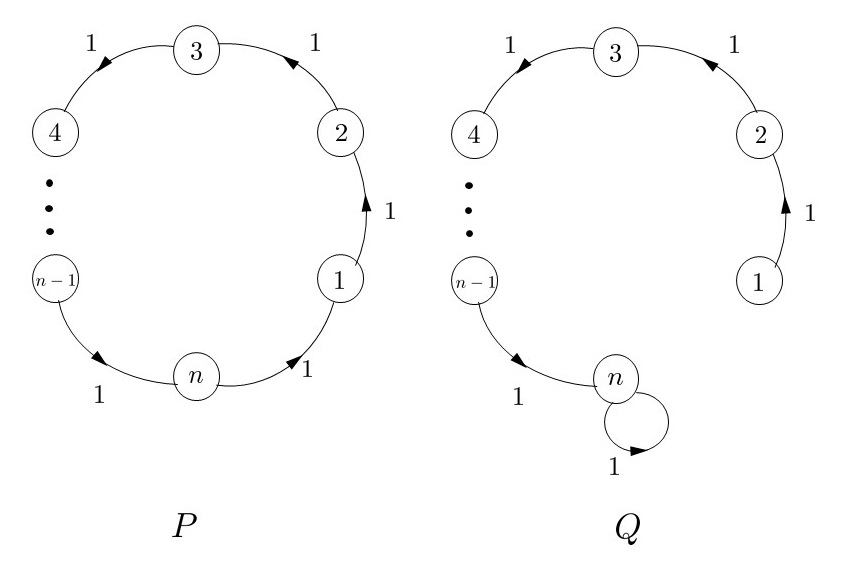
\includegraphics[scale=0.40]{diagrams/example2.jpg}
%	\caption{Example 2.}
%	\label{fig:example2}
%\end{figure}
%\end{example}
%
%\begin{example}
%\label{example:stationary_testing}
%Non symmetric MC: small difference between $P$ and $Q$ ($\dist{\word{P}{\ell}}{\word{Q}{\ell}}$ is small), but stationary distributions $\vect{p}_0$ and $\vect{q}_0$
%are vastly different. $Q$ - a ring with an edge $e=(v_1v_2)$ is removed, $v_1$ has a self-loop instead; $P$ - a similar ring with a loop, but $e$ is not removed but has a lighter
%weight of $\frac{1}{\sqrt{n}}$, while self-loop at $v_1$ has a weight of $1-\frac{1}{\sqrt{n}}$. Stationary distributions: $\vect{q}_0=\trans{(1,0,\cdots,0)}$ and
%$\vect{p}_0=\trans{(\frac{\sqrt{n}}{n+\sqrt{n}-1},\frac{1}{n+\sqrt{n}-1},\dots,\frac{1}{n+\sqrt{n}-1})}$, while $\specr{\srprod{P}{Q}}=\sqrt{1-\frac{1}{\sqrt{n}}}$.   
%%\begin{figure}[H]
%	%\centering
%		%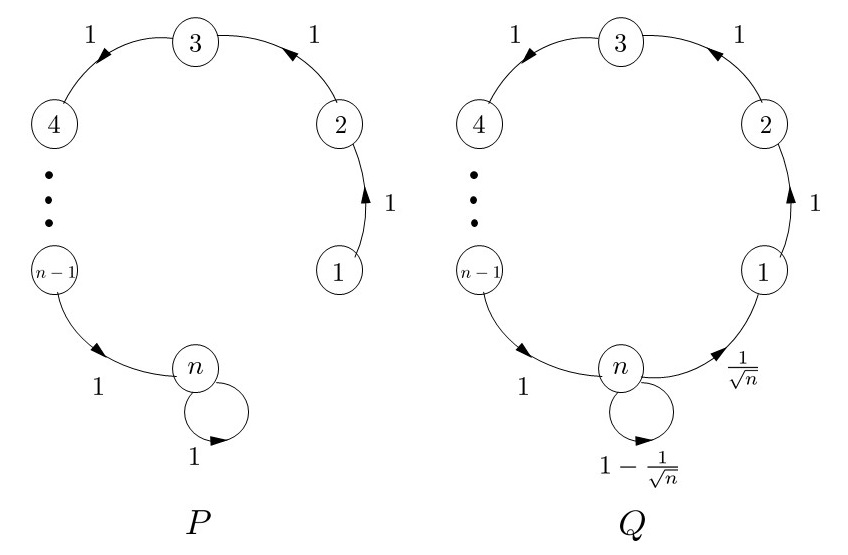
\includegraphics[scale=0.40]{diagrams/example3.jpg}
%	%\caption{Example 3.}
%	%\label{fig:example3}
%%\end{figure}
%
%\end{example}
%\begin{example}
%\label{example:same_stationary_large_dist}
%Non symmetric MC: same stationary (Uniform) distribution, $\dist{P}{Q}=1$, at average it takes $\Omega(n)$ steps to distinguish whether $P=Q$, or not.
%Two oriented cycles, 
%\[
%P\eqdef s_1\to s_2\to\cdots\to s_n\to s_1\quad\quad Q\eqdef s_1\to s_3\to s_4\cdots\to s_n\to s_2\to s_1.
%\]
%%\begin{figure}[H]
%	%\centering
%		%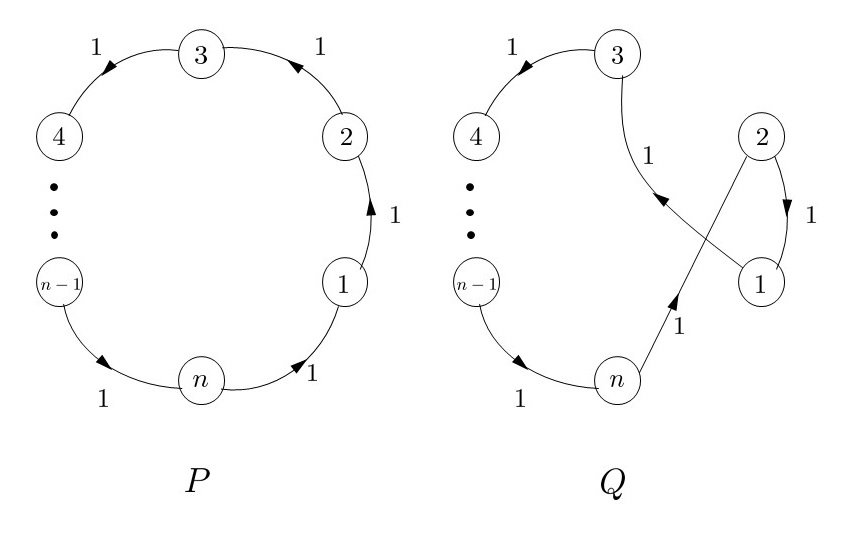
\includegraphics[scale=0.40]{diagrams/example4.jpg}
%	%\caption{Example 4.}
%	%\label{fig:example4}
%%\end{figure}
%\end{example}
%\begin{example}
%\label{example:symmetric}
%Symmetric Markov chains: $Q$ -- complete graph $Q_{ij}=1/n$; $P$ -- clique and disjoint vertex $P_{ij}=\frac{1}{n-1}, i,j\in[n-1]$, $P_{in}=P_{ni}=0, i\in[n-1],$ and 
%$P_{nn}=1$. Then $\eigi[1]=\sqrt{\frac{n-1}{n}}= 1 - \frac{1}{2n}+O(n^2)$, $\eigi[2]=\sqrt{\frac{1}{n}}$, $\eigi[3]=\cdots=\eigi[n]=0$. If Markov Chain starts from state $1$, 
%after one transition we would know almost certainly whether $w\sim P$, or $w\sim Q$. On the other hand, if $w$ starts from any other state, then it would take us about $n$ 
%observations to tell whether $w\sim P$, or $w\sim Q$. If we start from a random state, again we would need about $n$ steps to distinguish $P$ vs. $Q$.
%%\begin{figure}[H]
%	%\centering
%		%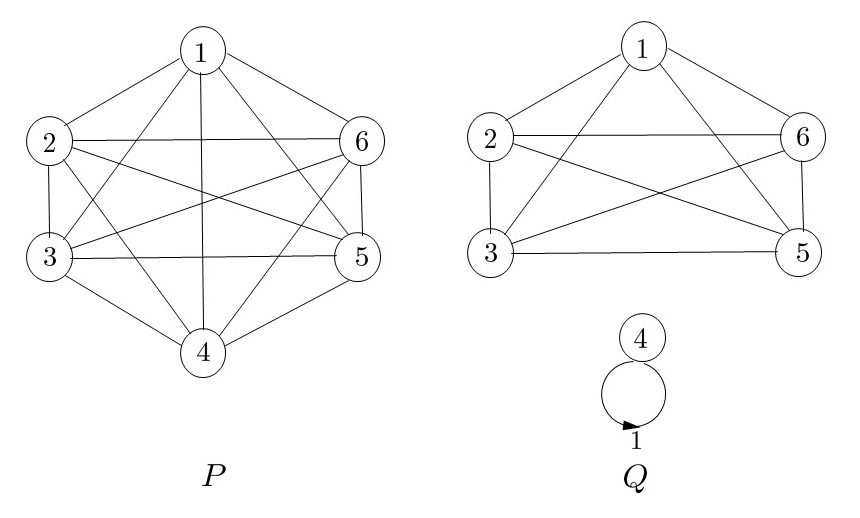
\includegraphics[scale=0.40]{diagrams/example5.jpg}
%	%\caption{Example 5.}
%	%\label{fig:example5}
%%\end{figure}
%\end{example}

